%!TEX root = ../GLM_Becerra_Lopez.tex

\section{Datos}
\label{sec:datos}

Los datos fueron obtenidos de Kaggle\footnote{\url{https://www.kaggle.com/new-york-city/nyc-property-sales}}, una plataforma de concursos de modelado predictivo y aprendizaje estadístico. Los datos de Kaggle, a su vez, provinieron de la página oficial del departamento de finanzas de la ciudad de Nueva York\footnote{\url{http://www1.nyc.gov/site/finance/taxes/property-rolling-sales-data.page}}.

Los datos tienen variables relacionadas con las casas y sus ventas, como distrito (\textit{borough}), vecindario (\textit{neighborhood}), código postal (\textit{zip code}), dirección, precio de venta del inmueble, fecha de venta, tipo de inmueble, tamaño del inmueble, etc. No se tiene información muy específica como número de cuartos o de baños.

Se tienen $84,548$ observaciones de un periodo de 12 meses (de septiembre de 2016 a agosto de 2017), las cuales no solo incluyen información de inmuebles residenciales, sino todo tipo de bienes raíces, por lo que se filtraron los datos para obtener solamente las observaciones correspondientes a casas. Además, había muchos datos que tenían como precio de venta 0, lo cual puede ser por herencia de padres a hijos o algún otro tipo de traspaso sin dinero\footnote{\url{http://www1.nyc.gov/assets/finance/downloads/pdf/07pdf/glossary_rsf071607.pdf}}. También existían ventas con valores no creíbles, como unos pocos miles de dólares, por lo que tampoco se tomaron en cuenta para este trabajo; además, también se filtraron las observaciones que no tenían información sobre el código postal. Después de este filtrado, quedaron $25,299$ observaciones.

En las siguientes subsecciones se muestra el análisis exploratorio de los datos.

\subsection{Gráficas univariadas}

La principal variable de interés es el precio en dólares de venta de las casas en Nueva York. En la figura \ref{fig:eda_histograma_precio_venta} se muestra una gráfica de frecuencias absoluta con y sin la transformación logaritmo. Como se puede observar, los precios de venta se asemejan a una distribución exponencial o gamma, pero aplicando la transformación logaritmo, los datos se asemejan a una muestra de una distribución normal, por lo que se usará esta transformación en los modelos posteriores.

\begin{figure}[H]
    \centering
    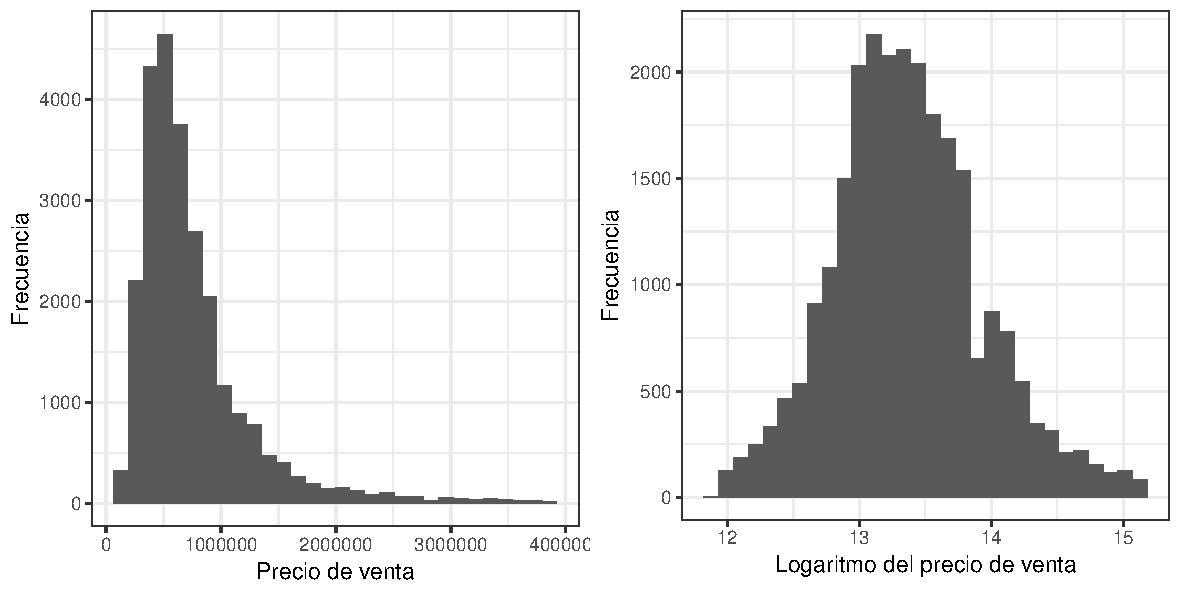
\includegraphics[width=0.9\textwidth]{images/eda_histograma_precio_venta.pdf}
    \caption{Histogramas del precio de venta en escala original y en escala logarítmica}
    \label{fig:eda_histograma_precio_venta}
\end{figure}


Otra de las variables de interés es la superficie total que esta medida en pies cuadrados. La figura \ref{fig:eda_histograma_superficie} muestra las gráficas de frecuencias absolutas para esta variable con y sin transformación logaritmo. De igual manera que el precio de ventas, sería más conveniente usar los datos usando la transformación logaritmo pues muestran un comportamiento semejante a una muestra de una distribución normal.

\begin{figure}[H]
    \centering
    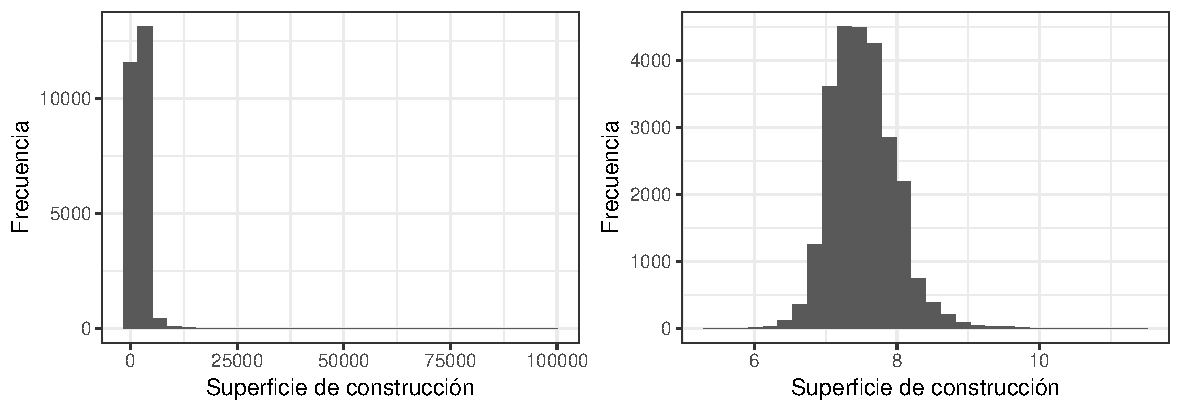
\includegraphics[width=0.9\textwidth]{images/eda_histograma_superficie.pdf}
    \caption{Histogramas de la superficie de construcción en escala original y en escala logarítmica}
    \label{fig:eda_histograma_superficie}
\end{figure}


Finalmente, la variable de superficie del terreno en pies cuadrados se muestra en la figura \ref{fig:eda_histograma_superficie_total_land}. En este caso también sería conveniente usar la transformación logaritmo en los datos pues mejora la distribución muestral y reescala los datos a una escala más pequeña.

\begin{figure}[H]
    \centering
    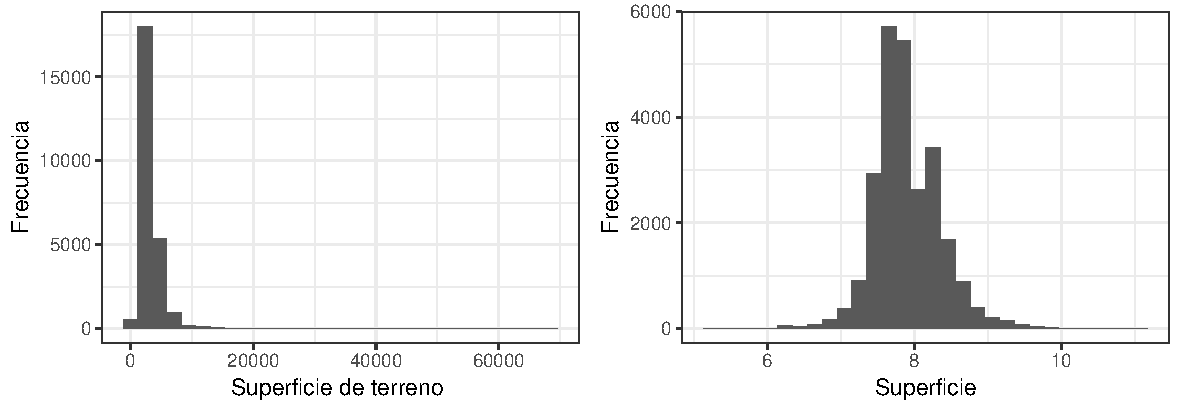
\includegraphics[width=0.9\textwidth]{images/eda_histograma_superficie_total_land.pdf}
    \caption{Histogramas de la superficie del terreno en escala original y en escala logarítmica}
    \label{fig:eda_histograma_superficie_total_land}
\end{figure}






\subsection{Gráficas bivariadas}

Primero se analizará la posible relación entre el precio de venta y la superficie total mediante un diagrama de dispersión. En la figura \ref{fig:eda_dispersion_superficie_vs_precio} se puede ver la gráfica de dispersión de la superficie de construcción contra el precio. Existe una tendencia lineal creciente entre las dos variables, es decir, a mayor superficie total también se tiene un mayor precio de venta. Por lo que la variable de superficie total puede ser usada como variable explicativa en un modelo de regresión.

\begin{figure}[H]
    \centering
    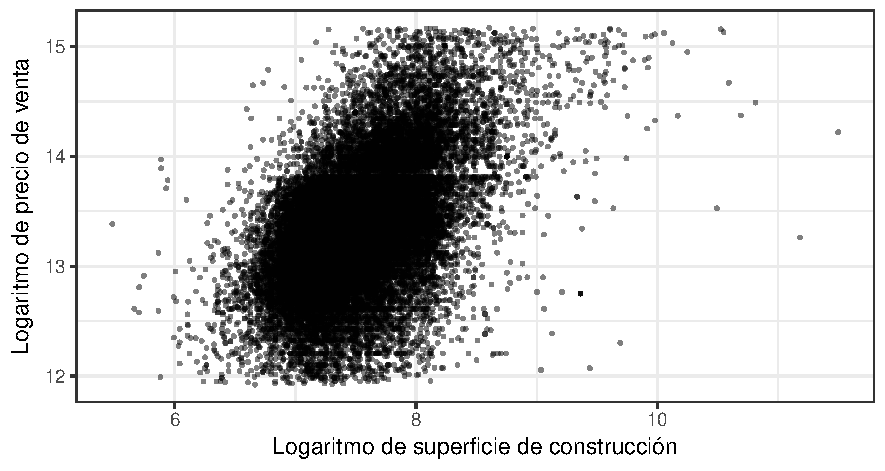
\includegraphics[width=0.7\textwidth]{images/eda_dispersion_superficie_vs_precio.pdf}
    \caption{Gráfica de dispersión de superficie de construcción contra precio}
    \label{fig:eda_dispersion_superficie_vs_precio}
\end{figure}


La relación entre la superficie de terreno y el precio de venta se muestra en el diagrama de dispersión de la figura \ref{fig:eda_dispersion_superficie_total_vs_precio}. Visualmente no existe una relación entre estas dos variables pues no muestra alguna tendencia. En la figura \ref{fig:eda_dispersion_superficie_total_vs_superficie} se muestra la posible relación entre las covariables superficie de construcción y superficie de terreno. Como es de esperarse, estas dos variables están relacionadas pues se puede esbozar una relación creciente, es decir, a mayor superficie total se tiene mayor superficie. Dada esta colinealidad, en un modelo de regresión se debería de usar alguna de estas dos variables pues proporcionan la misma información. En el caso de este trabajo, se seleccionó la variable de superficie de construcción debido a su correlación con el precio.


\begin{figure}[H]
    \centering
    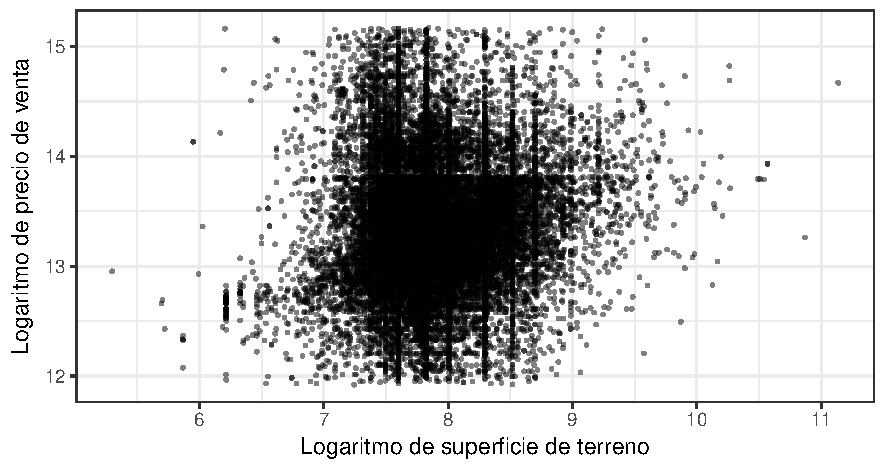
\includegraphics[width=0.7\textwidth]{images/eda_dispersion_superficie_total_vs_precio.pdf}
    \caption{Gráfica de dispersión de superficie de terreno contra precio}
    \label{fig:eda_dispersion_superficie_total_vs_precio}
\end{figure}


\begin{figure}[H]
    \centering
    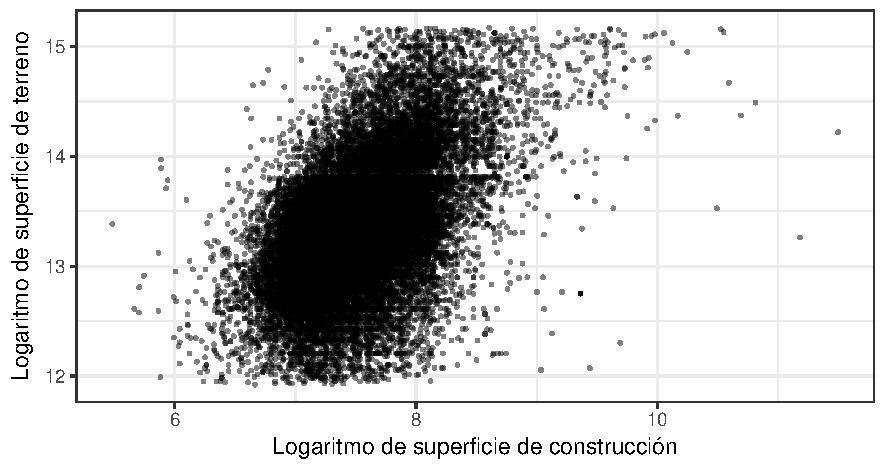
\includegraphics[width=0.7\textwidth]{images/eda_dispersion_superficie_total_vs_superficie.pdf}
    \caption{Gráfica de dispersión de superficie de construcción contra superficie del terreno}
    \label{fig:eda_dispersion_superficie_total_vs_superficie}
\end{figure}


Es de esperar que el precio de venta cambie dependiendo si la casa esta ubicada en cierto distrito (\textit{borough}). Para corroborar esta hipótesis se graficaron los precios en cada uno de los distritos, los cuales se pueden ver en las figuras \ref{fig:eda_histogram_price_borough} y \ref{fig:eda_boxplot_price_borough}. Se puede ver que, en efecto, cambian las distribuciones muestrales dependiendo el distrito en el que se encuentran las casas. También se puede ver que Manhattan muestra una media más alta que el resto de los distritos (línea punteada en figura \ref{fig:eda_boxplot_price_borough}), y también presenta más variación en los precios de venta. El siguiente distrito con una media más alta es Brooklyn con una variación más grande que el resto de los distritos (sin considerar Manhattan). 

\begin{figure}[H]
    \centering
    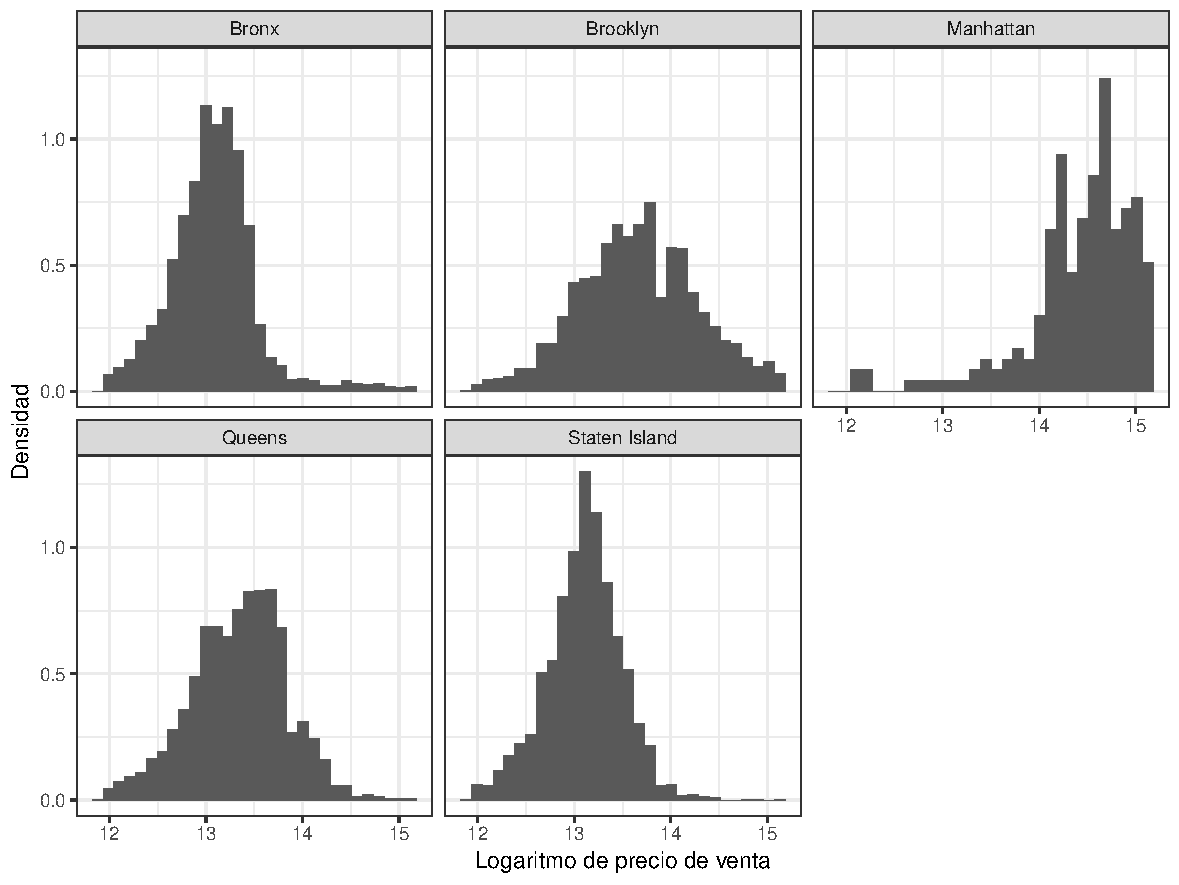
\includegraphics[width=0.7\textwidth]{images/eda_histogram_price_borough.pdf}
    \caption{Histogramas de precio de venta por distrito}
    \label{fig:eda_histogram_price_borough}
\end{figure}


\begin{figure}[H]
    \centering
    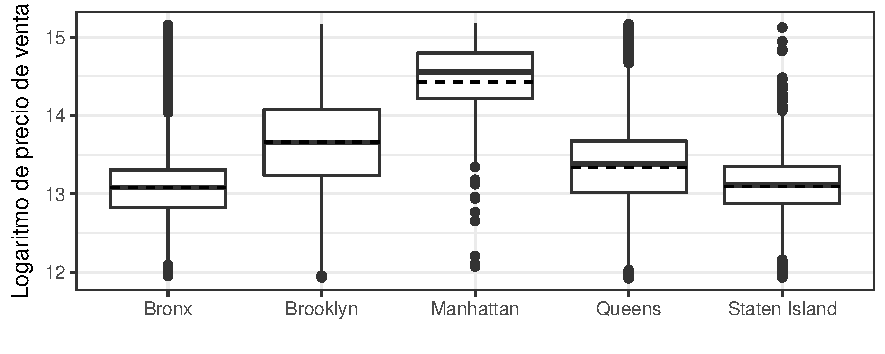
\includegraphics[width=0.7\textwidth]{images/eda_boxplot_price_borough.pdf}
    \caption{Diagrama de caja y brazos de precio de venta por distrito}
    \label{fig:eda_boxplot_price_borough}
\end{figure}

 

Hasta este momento se ha omitido la variable vecindario en el análisis exploratorio. La figura \ref{fig:eda_scatter_by_neighborhood} muestra la dispersión de los datos en cada vecindario. Se puede observar que considerando los vecindarios dentro de cada distrito, en algunos la relación creciente no es tan clara, o incluso llega a verse decreciente, como en el Upper West Side de Manhattan. Hay que tomar en cuenta que el número de observaciones en este vecindario es más pequeño. %Por ejemplo, en el distrito de Queens, los vecindarios Southeast Queens y Rockaways. Sin embargo los datos parecen seguir agrupandose por el tipo de casa que es. Tambien se puede observar que no en todas los vecindarios se encuentran todos los tipos de casas.

El propósito de esta gráfica es mostrar que las relaciones cambian de vecindario a vecindario, por lo que hay que tomar esto en cuenta al momento de hacer los modelos. Aún cuando existe otro nivel geográfico (los códigos postales), no es factible graficar la relación a este nivel pues son demasiados para que se pueda ver en una hoja, sin embargo, se hizo un análisis y también se ve que las relaciones cambian.

\begin{figure}[H]
    \centering
    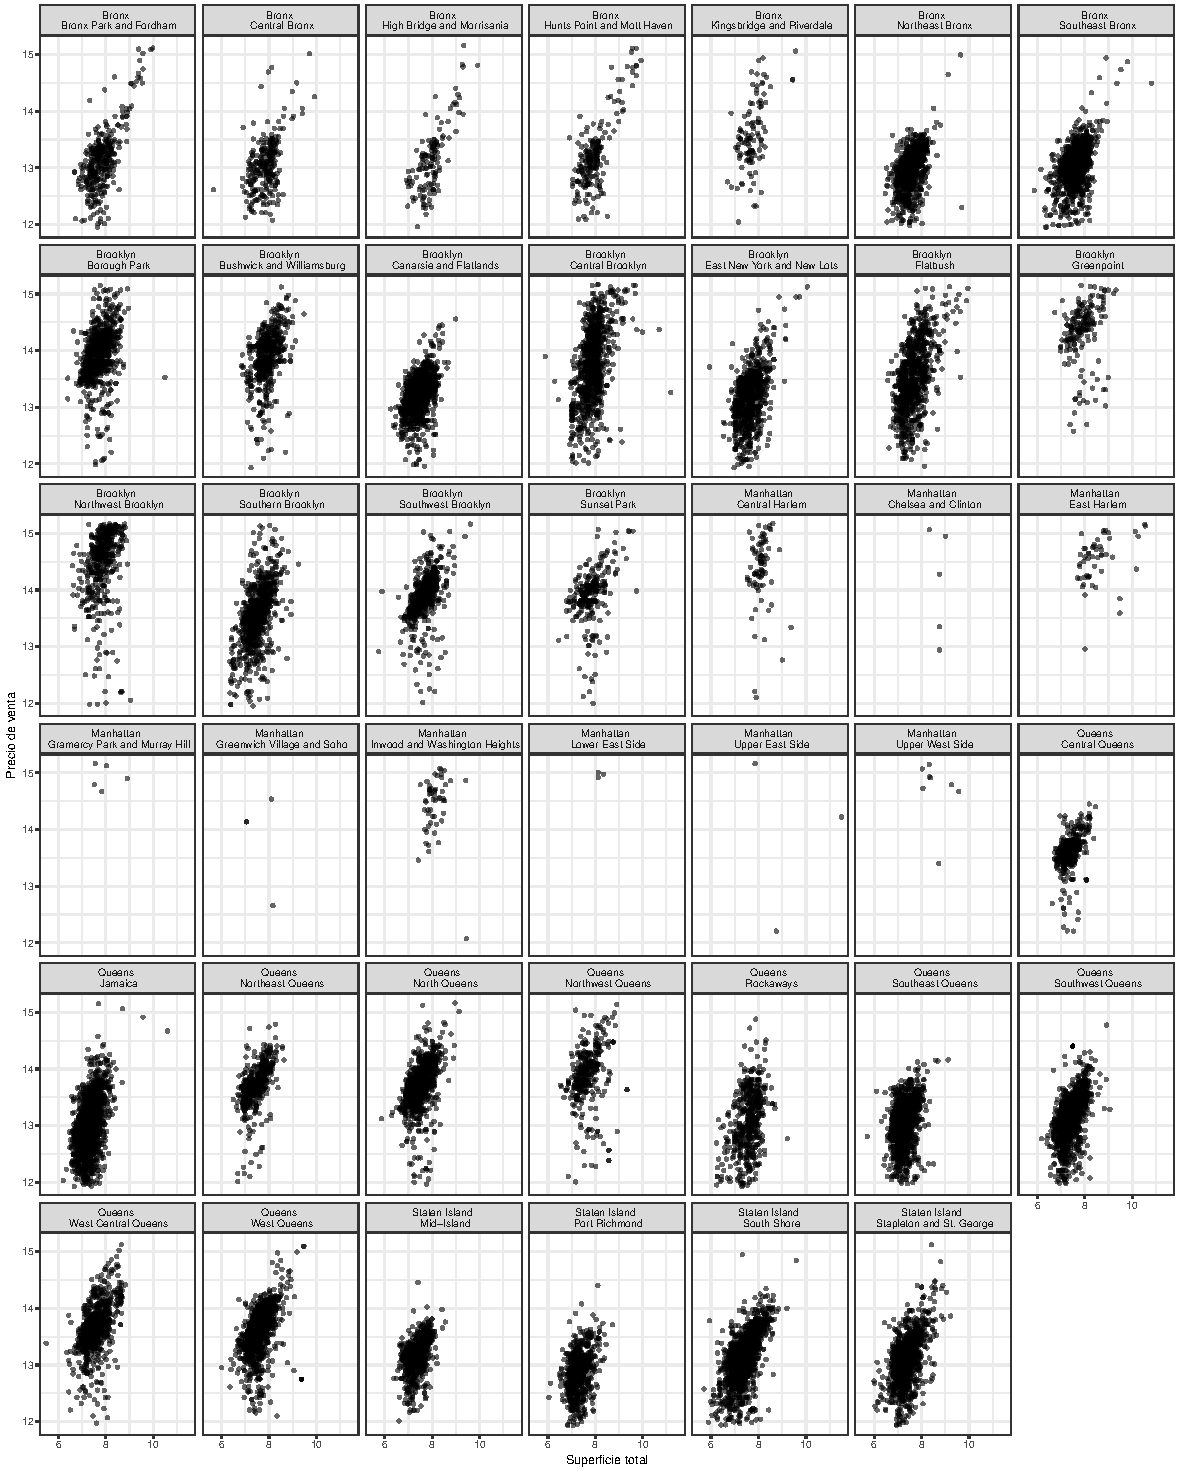
\includegraphics[width=1.03\textwidth]{images/eda_scatter_by_neighborhood.pdf}
    \caption{Diagramas de dispersión del logaritmo del precio contra el logaritmo del tamaño en cada vecindario}
    \label{fig:eda_scatter_by_neighborhood}
\end{figure}

